
\documentclass[11pt, a4paper]{book}
% Ressources à installer : texlive-science et texlive-lang-french ou texlive-lang-european
%à compiler avec XeLaTeX à cause des image pstricks

\usepackage[utf8]{inputenc}
\usepackage[T1]{fontenc}

\usepackage[french]{babel}
\usepackage{listingsutf8}
\usepackage{pdfpages}
\usepackage{tikz,pgf}
\usepackage{amsthm,titlesec}
\usepackage{mdframed} % pour le format des définition, théorèmes...
\usepackage{xcolor,rotating,systeme}
\usepackage[Glenn]{fncychap} %pour le format des chapitres
\usepackage[top=3cm,bottom=3cm,left=3cm,right=2cm,headsep=10pt,a4paper]{geometry} % Page margins
\usepackage{multicol}
\usepackage{comment}
\usepackage{enumerate,cancel}
\usepackage{lipsum,minitoc}
%\usepackage{chngcntr}
\usepackage{amsmath,amsfonts,minitoc,amsthm,pgfplots}
\usepackage{mathrsfs}
\usetikzlibrary{arrows, intersections}
\usepackage{mathrsfs}
\usepackage{array,yhmath}
\usepackage{hyperref}
\usepackage{caption}
\usepackage{float}
\usepackage{wrapfig}
\restylefloat{figure}
%\usepackage{subfig}

\usepackage{subcaption}

\usepackage{listings}
\usepackage{color}
\lstset{ % General setup for the package
    language=Python,
    basicstyle=\footnotesize,
    basewidth=0.7em,
    numbers=left,
     numberstyle=\tiny,
    frame=lines,
    tabsize=4,
    columns=fixed,
    showstringspaces=false,
    showtabs=false,
    keepspaces,
    commentstyle=\color{gray},
    keywordstyle=\color{blue},
    stringstyle=\color{magenta},
    inputencoding=utf8/latin1,
            extendedchars=true,
            literate=%
            {é}{{\'{e}}}1
            {è}{{\`{e}}}1
            {ê}{{\^{e}}}1
            {ë}{{\¨{e}}}1
            {û}{{\^{u}}}1
            {ù}{{\`{u}}}1
            {â}{{\^{a}}}1
            {à}{{\`{a}}}1
            {î}{{\^{i}}}1
            {ô}{{\^{o}}}1
            {ç}{{\c{c}}}1
            {Ç}{{\c{C}}}1
            {É}{{\'{E}}}1
            {Ê}{{\^{E}}}1
            {À}{{\`{A}}}1
            {Â}{{\^{A}}}1
            {Î}{{\^{I}}}1
    }



\usepackage{lipsum}
\newtheorem{example}{Exemple}

\usepackage{pstricks,pst-plot,pstricks-add}
\usepackage{pst-func,tkz-tab,tkz-euclide}
\usepackage{graphicx}
%macro exo
\newcounter{mtex}[chapter]
\newcommand{\mtexlabel}{\cadrexo{\themtex}}
\newcommand{\cadrexo}[1]{%
\tikz\node[rectangle,minimum size=6mm,rounded corners=2mm,fill=ocre,inner sep=0pt,text width=0.8cm,align=center]{\large\bfseries\textcolor{white}{#1}};}
\definecolor{ocre}{RGB}{196,106,106}
\definecolor{vert}{RGB}{55,120,0}
\newcommand{\mtexlabelpos}[1]{%
\makebox[0pt][r]{\raisebox{#1\baselineskip}[0pt][0pt]{\mtexlabel\quad}}}
\newenvironment{exercice}[1][\empty]{%
\refstepcounter{mtex}%
\trivlist\item\relax%  
\ifx#1\empty\mtexlabelpos{-.7}\else\mtexlabelpos{-.5}%
\hfill\textbf{#1}\hfill\mbox{}\par\fi%
}{\endtrivlist}

\newcommand{\N}{\mathbb{N}}
\newcommand{\Z}{\mathbb Z}
\newcommand{\Q}{\mathbb Q}
\newcommand{\R}{\mathbb R}
\newcommand{\C}{\mathbb C}

\newcommand{\ssi}{\;\;\Leftrightarrow\;\;}

\newcommand{\point}[1]{-- +(#1,#1) -- +(-#1,-#1) -- +(0,0) -- +(-#1,#1) -- +(#1,-#1)} 


\newcommand{\parallele}{\mathbin{\!/\mkern-5mu/\!}} %signe parallèle

\titleformat{\chapter}[frame]
{\setlength\fboxrule{2.25pt}\color{black}}%
{\filleft\scshape\LARGE%
\enspace  Chapitre \thechapter\enspace}%
{20pt}
{\rule{0pt}{30pt}\Huge\scshape\filleft}

\newcommand\fonction[5]{
$\begin{array}{rrll}
#1: & #2 & \rightarrow & #3 \\
  & #4 & \mapsto & #5
\end{array}$
}

%\titleformat
%{\section} % command
%[hang] % shape
%{\bfseries\Large} % format
%{ \thesection\quad} % label
%{0em} % sep
%{
%} % before-code
%[
%\vspace{-1ex}%
%\textcolor{blue!60}{\rule{10cm}{3pt}}
%] % after-code


%\theoremstyle{break}
\newtheoremstyle{definition-style}  %style des theoreme
{}               
{}               
{}                   
{}                   
{\bf\sffamily} 
{~:\\[0.3cm]}                 
{.5em}               
{\thmname{#1}\thmnumber{ #2}\thmnote{ (#3)}}

\mdfdefinestyle{defi-frame}{
linewidth=10pt, %
linecolor= blue!50, % 
backgroundcolor= blue!20,
topline=false, %
bottomline=false, %
rightline=false,%
leftmargin=0pt, %
innerleftmargin=15pt, %
innerrightmargin=1em, 
rightmargin=0pt, % 
innertopmargin=-2pt,%
innerbottommargin=6pt, % 
splittopskip=\topskip, %
%splitbottomskip=\topskip, %
}% 

\mdfdefinestyle{methode-frame}{
	linewidth=10pt, %
linecolor= gray!70, % 
backgroundcolor= white,
topline=false, %
bottomline=false,%
rightline=false,%
leftmargin=0pt, %
innerleftmargin=15pt, %
innerrightmargin=1em, 
rightmargin=0pt, % 
innertopmargin=-2pt,%
innerbottommargin=6pt, % 
splittopskip=\topskip, %
%splitbottomskip=\topskip, %
}% 


\mdfdefinestyle{thm-frame}{
linewidth=10pt, %
linecolor= red!50, % 
backgroundcolor= orange!30,
topline=false, %
bottomline=false, %
rightline=false,%
leftmargin=0pt, %
innerleftmargin=15pt, %
innerrightmargin=1em, 
rightmargin=0pt, % 
innertopmargin=-2pt,%
innerbottommargin=6pt, % 
splittopskip=\topskip, %
%splitbottomskip=\topskip, %
}% 

\mdfdefinestyle{lem-frame}{
linewidth=10pt, %
linecolor= yellow!50, % 
backgroundcolor= yellow!10,
topline=false, %
bottomline=false, %
rightline=false,%
leftmargin=0pt, %
innerleftmargin=15pt, %
innerrightmargin=1em, 
rightmargin=0pt, % 
innertopmargin=-2pt,%
innerbottommargin=6pt, % 
splittopskip=\topskip, %
%splitbottomskip=\topskip, %
}% 

\mdfdefinestyle{notation-frame}{
linewidth=10pt, %
linecolor= blue!30, % 
backgroundcolor= blue!10,
topline=false, %
bottomline=false, %
rightline=false,%
leftmargin=0pt, %
innerleftmargin=15pt, %
innerrightmargin=1em, 
rightmargin=0pt, % 
innertopmargin=-2pt,%
innerbottommargin=6pt, % 
splittopskip=\topskip, %
%splitbottomskip=\topskip, %
}% 

\mdfdefinestyle{remarque-frame}{
linewidth=0pt, %
linecolor= black!0, % 
backgroundcolor= blue!0,
topline=false, %
bottomline=false, %
rightline=false,%
leftmargin=0pt, %
innerleftmargin=25pt, %
innerrightmargin=25pt, 
rightmargin=0pt, % 
innertopmargin=-2pt,%
innerbottommargin=6pt, % 
splittopskip=\topskip, %
%splitbottomskip=\topskip, %
}% 
\surroundwithmdframed[style=defi-frame]{defi}

\surroundwithmdframed[style=thm-frame]{thm}

\surroundwithmdframed[style=lem-frame]{lem}

\surroundwithmdframed[style=notation-frame]{notation}

\surroundwithmdframed[style=remarque-frame]{remarque}

\surroundwithmdframed[style=remarque-frame]{remarques}

\surroundwithmdframed[style=methode-frame]{methode}

\theoremstyle{definition-style}

%pour avoir un compteur commun a remarque et remarques
\newcounter{compteurremarque}[chapter]
\renewcommand{\thecompteurremarque}{\arabic{compteurremarque}} %définition de l'affichage du compteur

\newtheorem{defi}{Définition}[chapter]
\renewcommand{\thedefi}{\arabic{defi}} %pour ne pas avoir le numéro du chapitre dans la numération de la def
\newtheorem{thm}{Théorème}[chapter]
\renewcommand{\thethm}{\arabic{thm}}
\newtheorem{lem}{Lemme}[chapter]
\renewcommand{\thelem}{\arabic{lem}}
\newtheorem{notation}{Notation}[chapter]
\renewcommand{\thenotation}{\arabic{notation}}
%\newtheorem{remarque}{Remarque}[chapter]
%\renewcommand{\theremarque}{\arabic{remarque}}
%\newtheorem{remarques}{Remarques}[chapter]
%\renewcommand{\theremarques}{\arabic{remarques}}
\newtheorem{methode}{Méthode}[chapter]
\renewcommand{\themethode}{\arabic{methode}}


\newtheorem{remarque}[compteurremarque]{Remarque}
\newtheorem{remarques}[compteurremarque]{Remarques} %remarque et remarques prennent compteurremarque comme compteur commun

\lstMakeShortInline[columns=fixed]|

%%%%%%%% Commandes de Matthieu

%-------------------------------------------------------------------------------
%---- Eclairage : en encadré sur fond jaune avec symbôle "ampoule" à gauche ----
%-------------------------------------------------------------------------------
\definecolor{coleclairage}{RGB}{255 , 221 , 156}
\definecolor{contoureclairage}{RGB}{255 , 192 , 0}
\newenvironment{eclairage}
{
	\begin{center}%
		\begin{tikzpicture}%
			\node[rectangle, draw=contoureclairage, top color=coleclairage!50, bottom color=coleclairage!140, rounded corners=5pt, inner xsep=5pt, inner ysep=6pt, outer ysep=10pt]\bgroup                     
			\begin{minipage}{0.98\linewidth}
				\begin{minipage}{0.08\linewidth}\centerline{
\includegraphics[scale=1]{images/Symbole_eclairage.png}}\end{minipage}
				\begin{minipage}{0.89\linewidth}\itshape\footnotesize
				}
				{                		
				\end{minipage}
			\end{minipage}\egroup;%
		\end{tikzpicture}%
	\end{center}%
}



\newcommand{\putfigure}[6]{
    \begin{minipage}{#1\textwidth}
    \centering
        \includegraphics[width=#2\textwidth,height=#3\textheight]{#4}
        \captionof{figure}{#5}
        \label{#6}
    \end{minipage}
}


\newcommand{\itemb}[1]{\item \textbf{#1}}



%-------------------------------------------------------------------------------
%---- apprendre : en encadré sur fond jaune avec symbole "ampoule" à gauche ----
%-------------------------------------------------------------------------------
\definecolor{colapprendre}{RGB}{50,205,50}
\definecolor{contourapprendre}{RGB}{34,139,34}
\newenvironment{apprendre}
{
	\begin{center}%
		\begin{tikzpicture}%
			\node[rectangle, draw=contourapprendre, top color=colapprendre!10, bottom color=colapprendre!50, rounded corners=5pt, inner xsep=5pt, inner ysep=6pt, outer ysep=10pt]\bgroup                     
			\begin{minipage}{0.98\linewidth}
				\begin{minipage}{0.08\linewidth}\centerline{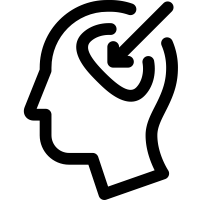
\includegraphics[width=30px]{images/Symbole_learn.png}}\end{minipage}
				\begin{minipage}{0.89\linewidth}\itshape\footnotesize
				}
				{                		
				\end{minipage}
			\end{minipage}\egroup;%
		\end{tikzpicture}%
	\end{center}%
}

\definecolor{colimportant}{RGB}{247 , 189 , 164}
\definecolor{contourimportant}{RGB}{237 , 125 , 49}
\newenvironment{important}
{
	\begin{center}%
		\begin{tikzpicture}%
			\node[rectangle, draw=contourimportant, top color=colimportant!50, bottom color=colimportant!140, rounded corners=5pt, inner xsep=5pt, inner ysep=6pt, outer ysep=10pt]\bgroup                     
			\begin{minipage}{0.08\linewidth}\centerline{
\includegraphics[scale=0.8]{images/Symbole_attention.png}}\end{minipage}
			\begin{minipage}{0.89\linewidth}
			}
			{                		
			\end{minipage}\egroup;
		\end{tikzpicture}%
	\end{center}%
}

%----------------------------------------------
\newcounter{compteurmonprogramme}
\setcounter{compteurmonprogramme}{1}
\newenvironment{monprogramme}
{
	\begin{center}%
		\begin{tikzpicture}%
			\node[rectangle, draw=black, rounded corners=5pt, inner xsep=5pt, inner ysep=6pt, outer ysep=10pt]\bgroup                     
			\begin{minipage}{0.98\linewidth}
				{\bf Programme \thechapter.\thecompteurmonprogramme\;:}
				
				\vspace{2mm}\hspace{7.5mm}
				\begin{minipage}{0.93\linewidth}
				}
				{                		
				\end{minipage}
				\stepcounter{compteurmonprogramme}
			\end{minipage}\egroup;%
		\end{tikzpicture}%
	\end{center}%
}



%------------------------------------------------
%---- Définition : en encadré sur fond blanc ----
%------------------------------------------------
\newcounter{compteurdef}
\setcounter{compteurdef}{1}
\newenvironment{mydefinition}
{
	\begin{center}%
	\begin{tikzpicture}%
		\node[rectangle, draw=black, rounded corners=5pt, inner xsep=5pt, inner ysep=6pt, outer ysep=10pt]\bgroup                    
		\begin{minipage}{0.98\linewidth}
			{\bf {\underline {Définition \thechapter.\thecompteurdef}}}
			
			\vspace{2mm}\hspace{4.5mm}
			\begin{minipage}{0.93\linewidth}
			}
			{                		
			\end{minipage}
			\stepcounter{compteurdef}
		\end{minipage}\egroup;%
	\end{tikzpicture}%
\end{center}%
}

\newenvironment{mydefinitions}
{
	\begin{center}%
		\begin{tikzpicture}%
			\node[rectangle, draw=black, rounded corners=5pt, inner xsep=5pt, inner ysep=6pt, outer ysep=10pt]\bgroup                    
			\begin{minipage}{0.98\linewidth}
				{\bf {\underline {Définitions \thechapter.\thecompteurdef}}}
				
				\vspace{3mm}\hspace{4.5mm}
				\begin{minipage}{0.93\linewidth}\slshape
					\begin{itemize}\setlength{\itemsep}{1mm}
					}
					{                		
				\end{itemize}\end{minipage}
				\stepcounter{compteurdef}
			\end{minipage}\egroup;%
		\end{tikzpicture}%
	\end{center}%
}



%------------------------------------------------
%---- Exemple : en encadré sur fond blanc ----
%------------------------------------------------
\newcounter{compteurex}
\setcounter{compteurex}{1}
\newenvironment{myexample}{
	\begin{center}
	\vspace{-3mm}
	\begin{minipage}{1\linewidth}
		\vspace{2mm}
		{\textsl {\underline {Exemple \thechapter.\thecompteurex}}}
		
		\vspace{2mm}\hspace{2.5mm}
		\begin{minipage}{1\linewidth}
			\begin{mdframed}[topline=false,rightline=false,bottomline=false]
}
{
			\end{mdframed}
		\end{minipage}
		\stepcounter{compteurex}
	\end{minipage}
	\end{center}
}
\newenvironment{myexamples}{
	\begin{center}
		\vspace{-3mm}
		\begin{minipage}{1\linewidth}
			\vspace{2mm}
			{\textsl {\underline {Exemples \thechapter.\thecompteurex}}}
			
			\vspace{2mm}\hspace{2.5mm}
			\begin{minipage}{1\linewidth}%\slshape
				\begin{mdframed}[topline=false,rightline=false,bottomline=false]
					\begin{enumerate}\setlength{\itemsep}{1mm}
				}
				{
					\end{enumerate}
				\end{mdframed}
			\end{minipage}
			\stepcounter{compteurex}
		\end{minipage}
	\end{center}
}



\newtheorem*{question}{Question}



%%%%%%%%%%%%%%%%%%%%%%%%%%%%%%%%%%%%%%%%%%%%%%%%%%%%%%%%%%%%%%%%%%%%%%%%%%%%
%%%%%%%%%%%%%%%%%%%%%%%%%%%   LABELS activite   %%%%%%%%%%%%%%%%%%%%%%%%%%%
%%%%%%%%%%%%%%%%%%%%%%%%%%%%%%%%%%%%%%%%%%%%%%%%%%%%%%%%%%%%%%%%%%%%%%%%%%%%
\newcommand{\act}{\textbf{\textsl{Activité \arabic{compteuract}}} \vspace*{1mm}\\ \addtocounter{compteuract}{1}}
\newcommand{\actnomme}[1]{{\bf Activité \arabic{compteuract} {\textsl{\small (#1)}}}\vspace*{1mm}\\  \addtocounter{compteuract}{1}}
\newcounter{compteuract}
\setcounter{compteuract}{1}
\newcommand{\getactcompteur}{{\the\numexpr \arabic{compteuract} - 1 \relax}}



%%%%%%%%%%%%%%%%%%%%%%%%%%%%%%%%%%%%%%%%%%%%%%%%%%%%%%%%%%%%%%%%%%%%%%%%%%%%
%%%%%%%%%%%%%%%%%%%%%%%%%%%   LABELS EXERCICES   %%%%%%%%%%%%%%%%%%%%%%%%%%%
%%%%%%%%%%%%%%%%%%%%%%%%%%%%%%%%%%%%%%%%%%%%%%%%%%%%%%%%%%%%%%%%%%%%%%%%%%%%
\newcommand{\exo}{\textbf{\textsl{Exercice \arabic{compteurexo}}} \vspace*{1mm}\\ \addtocounter{compteurexo}{1}}
\newcommand{\exonomme}[1]{{\bf Exercice \arabic{compteurexo} {\textsl{\small (#1)}}}\vspace*{1mm}\\  \addtocounter{compteurexo}{1}}
\newcommand{\eexo}{\vspace{5mm}} % espace pour séparer les exercices
\newcounter{compteurexo}
\setcounter{compteurexo}{1}
\newcommand{\getexocompteur}{{\the\numexpr \arabic{compteurexo} - 1 \relax}}
\pgfplotsset{compat=1.17}
\begin{document}

\setcounter{chapter}{1}
\chapter{Représentation numérique de l’information - Images}

\subsection{Image numérique}

Grâce aux nombres, les ordinateurs stockent des dessins, des photos et d’autres types d’images.
{\it Wikipedia} définit l'image numérique  comme toute image (dessin, icône, photographie…) acquise, créée, traitée et stockée sous forme binaire.

On distingue deux types d’images numériques:
\begin{enumerate}[a)]
\item {\bf L'image matricielle (ou bitmap)}:
Elle est composée de points appelés pixels que l’on ne voit pas à l'œil nu. Lors de l’agrandissement, l’image peut devenir floue, car les pixels ressortent ( les carrés sur l’écran).
\item {\bf L'image vectorielle}:
Elle est composée de lignes et de segments qui sont liés entre eux par des formules mathématiques. Grâce à la vectorisation, chaque élément a une place définie qui empêche la déformation de l’image. Au lieu de mémoriser une mosaïque de points élémentaires, on stocke la succession d’opérations conduisant au tracé.

L’usage de ce type d’image concerne les schémas générés par certains logiciels de DAO (Dessin assisté par ordinateur) ou pour les animations Flash utilisées sur internet pour la création de bannières publicitaires.

\end{enumerate}

\begin{center}
\begin{figure}
\centering
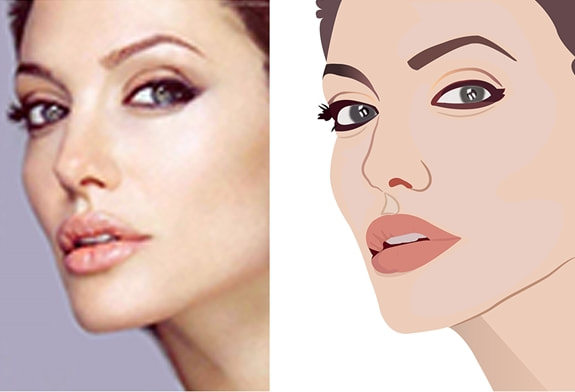
\includegraphics[width=8cm]{images/bitmapvectoriel}
\caption{Différence entre une image bitmap (à gauche) et vectorielle (à droite)}
\end{figure}
\end{center}

\begin{remarque}

Il n’est pas possible de tout vectoriser, car les photos et les dégradés de couleurs ne se vectorisent pas. En effet, la vectorisation aplatit les couleurs et élimine des dégradés.

\end{remarque}

\subsection{Définition et Résolution}
Il est important de définir les notions suivantes : 
\subsubsection{Définition}
 La \textbf{définition} d'une image est le nombre de points (pixels) constituant l’image.
 
\subsubsection{Résolution}
 La \textbf{résolution} d'une image est le nombre de points par unité de surface, exprimé en points par pouce (PPP, en anglais DPI pour Dots Per Inch), un pouce représentant 2.54 cm.

\begin{center}
\begin{figure} [h!]
\centering
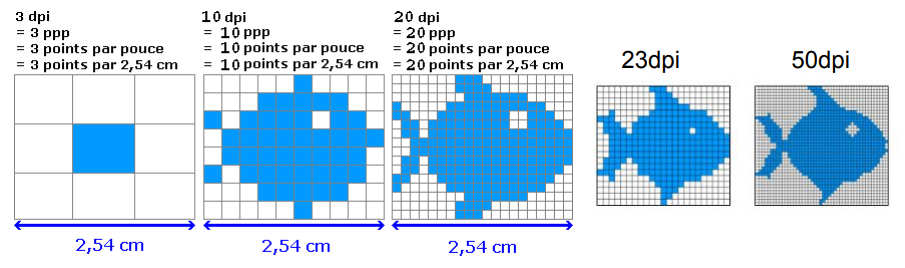
\includegraphics[width=8cm]{images/dpi_poisson.png}
\caption{Résolution d'une image}
\end{figure}
\end{center}

\subsubsection{Dimension}
La \textbf{dimension} d’une image est définie par:
$$largeur = nombre\ de\ colonnes / resolution$$
$$hauteur = nombre\ de\ ligne / resolution$$

Exemple: Une image de 1024x768 pixels avec une résolution de 300 dpi aura une:
$$largeur = 1024 / 300 = 3,41 pouces (8,66 cm)$$
$$hauteur = 768 / 300 = 2,56 pouces (6,5 cm)$$


\subsection{Coder une image en noir et blanc}

\subsubsection{Première méthode}

\begin{defi}
Les écrans d’ordinateur sont divisés en une grille de petits points appelés pixels (picture elements, qui signifie éléments d’image)
\end{defi}

Chaque pixel de l'image est codé soit par un 0, représentant un point noir ou un 1, représentant un point blanc. Donc, un bit permet de coder un pixel d’une image en noir et blanc. 

Pour stocker une image en noir et blanc, il suffit de convertir le noir par 0 et le blanc par 1. 

\begin{center}
\begin{tikzpicture}[scale=.5]
\foreach \x in {0,...,8}
	{\draw (0,\x) -- +(8,0);
	\draw (\x,0) -- +(0,8);
	}
\foreach \x in {0,...,7}{
	\foreach \y in {0,...,7}{
			\draw (\x+.5,\y+.5)  node {$1$};
		}
	}	
	
\foreach \x in {(2,0),(3,0),(5,0),(6,0),
						(3,1),(4,1),(5,1),
						(2,2),(3,2),(5,2),(6,2),
						(2,3),(3,3),(5,3),(6,3),
						(3,4),(4,4),(5,4),
						(4,5),
						(2,6),(3,6),(4,6),(5,6),
						(3,7),(4,7),(5,7)
						}{
		\filldraw[fill=black] \x rectangle +(1,1);
		\draw[color=white] \x +(.5,.5) node {0};
}
	
\end{tikzpicture}
\end{center}

\subsubsection{Deuxième méthode *}

Une autre façon consiste à indiquer pour chaque ligne le nombre de points blancs et de points noirs consécutifs.

\begin{center}
\begin{tikzpicture}[scale=.5]
\foreach \x in {0,...,5}
	{\draw (0,\x) -- +(5,0);
	\draw (\x,0) -- +(0,6);
	}
\draw (0,6) -- (5,6);
	
\foreach \x in {(1,0),(2,0),(3,0),(4,0),
						(0,1),(4,1),
						(0,2),(4,2),
						(1,3),(2,3),(3,3),(4,3),
						(4,4),
						(1,5),(2,5),(3,5)
						}{
		\filldraw[fill=black] \x rectangle +(1,1);
		
}
	
\draw (6,0.5) node[right] {1,4};	
\draw (6,1.5) node[right] {0,1,3,1};	
\draw (6,2.5) node[right] {0,1,3,1};	
\draw (6,3.5) node[right] {1,4};
\draw (6,4.5) node[right] {4,1};	
\draw (6,5.5) node[right] {1,3,1};		
	
\end{tikzpicture}
\end{center}

L’image de la lettre “a” nous montre comment une image peut être représentée par des nombres. Le premier nombre représente toujours le nombre de pixels blancs. Si le premier pixel est noir, la ligne commencera par un 0.
\begin{enumerate}[a)]
\item La première ligne est représentée par 1, 3, 1.
\item La première ligne contient 1 pixel blanc, 3 noirs, puis 1 blanc. 
\item La quatrième ligne est représentée par 0, 1, 3, 1.
\end{enumerate}

\vspace{2cm}
\begin{exercice}
Décoder l'image suivante:

\begin{center}
\begin{tikzpicture}[scale=.5]
\foreach \x in {0,...,17}{
	\draw (\x,0) -- +(0,13);
	}

\foreach \x in {0,...,13}{
	\draw (0,\x) -- +(17,0);
	}
\draw (17,12.5) node[right] {11111111111111111}; 
\draw (17,11.5) node[right] {11111110001110011}; 
\draw (17,10.5) node[right] {11111001110001101}; 
\draw (17,9.5) node[right] {11110111101101101}; 
\draw (17,8.5) node[right] {11110110011101011}; 
\draw (17,7.5) node[right] {11101001111110111}; 
\draw (17,6.5) node[right] {11100111111110111}; 
\draw (17,5.5) node[right] {11101111111110111}; 
\draw (17,4.5) node[right] {11010111111101111}; 
\draw (17,3.5) node[right] {10110111111101111}; 
\draw (17,2.5) node[right] {10111001110011111}; 
\draw (17,1.5) node[right] {11000110001111111}; 
\draw (17,0.5) node[right] {11111111111111111}; 	

\end{tikzpicture}
\end{center}
\end{exercice}


\begin{exercice}
Décoder l'image suivante: *

\begin{center}
\begin{tikzpicture}[scale=.5]
\foreach \x in {0,...,16}{
	\draw (\x,0) -- +(0,9);
	}

\foreach \x in {0,...,9}{
	\draw (0,\x) -- +(16,0);
	}

\draw (17,8.5) node[right] {4,11}; 
\draw (17,7.5) node[right] {4,9,2,1}; 
\draw (17,6.5) node[right] {4,9,2,1}; 
\draw (17,5.5) node[right] {4,11}; 
\draw (17,4.5) node[right] {4,9}; 
\draw (17,3.5) node[right] {4,9}; 
\draw (17,2.5) node[right] {5,7}; 
\draw (17,1.5) node[right] {0,16}; 
\draw (17,0.5) node[right] {1,14}; 	

\end{tikzpicture}
\end{center}
\end{exercice}


\subsection{Coder une image en niveaux de gris}

Plutôt que de simplement avoir 2 couleurs possibles, noir et blanc, on peut décider d'avoir N gris différents allant du plus sombre, le noir, au plus clair, le blanc.

Pour stocker une image en mémoire, il suffit de convenir que chaque point de l’image est représenté par un nombre. 

Ce dernier correspond à une certaine couleur.

Pour une image en 16 niveaux de gris, il faut que chaque point de l’image soit codé par un nombre en 4 bits.

Si chaque point est codé sur 8 bits, l’image peut contenir 256 niveaux de gris différents. Si l'on souhaite que l'image contienne plus de couleurs, on pourra utiliser plus de bits pour chaque pixel.


\begin{center}
\begin{figure}[H]
\centering
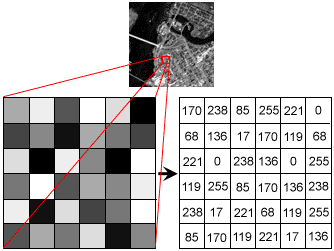
\includegraphics[width=8cm]{images/grayscale}
\caption{Image en niveaux de gris}
\end{figure}
\end{center}


\subsection{Coder une image en couleur}

Pour représenter des images avec des couleurs réalistes, on peut utiliser la même méthode que pour les niveaux de gris, mais en utilisant 3 nombres différents, 1 pour chaque couleur primaire.

Le code le plus utilisé est le codage {\bf RVB} (Rouge, Vert, Bleu) (RGB en anglais). 

Chacune de ces couleurs est codée sur 1 octet (8 bits). 
Avec ce système, chaque pixel est codé sur 3 octets pour un total de 24 bits. 

La valeur décimale pour chaque couleur peut s’étendre de 0 à 255, cette limite est fixée par la valeur maximale qu’un octet peut représenter avec le système binaire.

L’avantage du système RVB est sa simplicité, 
il s’appuie sur les caractéristiques de la vision humaine pour fournir à l’utilisateur une reproduction des couleurs au plus proche de la réalité.


\begin{center}
\begin{figure}[H]
\centering
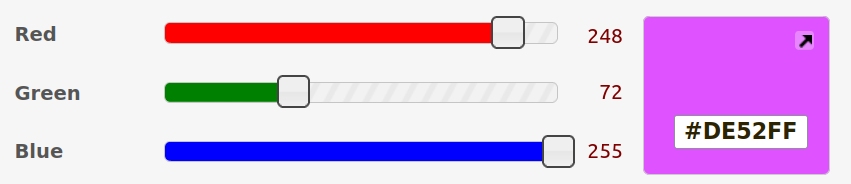
\includegraphics[width=8cm]{images/RGB}
\caption{Image RGB}
\end{figure}
\end{center}


\begin{center}
\begin{tikzpicture}[scale=.5]
\foreach \x in {0,...,10}{
	\draw (0,\x) -- +(30,0);
	} 

\draw (6,0) -- +(0,10);
\draw (14,0) -- +(0,10);
\draw (22,0) -- +(0,10);
\draw (30,0) -- +(0,10);
\draw (0,0) -- +(0,10);

\filldraw[fill=lightgray] (6,9) rectangle (30,10);

\draw (18,10.5) node {codage pixel en décimal};

\filldraw[fill=black] (0,0) rectangle (6,1);
\draw[white] (3,0.5) node {Noir};
\draw (10,0.5) node {0};
\draw (18,0.5) node {0};
\draw (26,0.5) node {0};

\definecolor{magenta}{rgb}{255,0,255}

\filldraw[fill=magenta] (0,1) rectangle +(6,1);
\draw (3,1.5) node {Magenta};
\draw (10,1.5) node {255};
\draw (18,1.5) node {0};
\draw (26,1.5) node {255};


\filldraw[fill=blue] (0,2) rectangle +(6,1);
\draw[white] (3,2.5) node {Bleu};
\draw (10,2.5) node {0};
\draw (18,2.5) node {0};
\draw (26,2.5) node {255};

\definecolor{cyan}{rgb}{0,255,255}

\filldraw[fill=cyan] (0,3) rectangle +(6,1);
\draw (3,3.5) node {Cyan};
\draw (10,3.5) node {0};
\draw (18,3.5) node {255};
\draw (26,3.5) node {255};

\filldraw[fill=green] (0,4) rectangle +(6,1);
\draw (3,4.5) node {Vert};
\draw (10,4.5) node {0};
\draw (18,4.5) node {255};
\draw (26,4.5) node {0};

\definecolor{jaune}{rgb}{255,255,0}

\filldraw[fill=jaune] (0,5) rectangle +(6,1);
\draw (3,5.5) node {Jaune};
\draw (10,5.5) node {255};
\draw (18,5.5) node {255};
\draw (26,5.5) node {0};

\filldraw[fill=red] (0,6) rectangle +(6,1);
\draw (3,6.5) node {Rouge};
\draw (10,6.5) node {255};
\draw (18,6.5) node {0};
\draw (26,6.5) node {0};

\filldraw[fill=white] (0,7) rectangle +(6,1);
\draw (3,7.5) node {Blanc};
\draw (10,7.5) node {255};
\draw (18,7.5) node {255};
\draw (26,7.5) node {255};

\filldraw[fill=gray] (0,8) rectangle +(6,1);
\draw (3,8.5) node {Gris moyen};
\draw (10,8.5) node {127};
\draw (18,8.5) node {127};
\draw (26,8.5) node {127};


\draw (3,9.5) node {\bf Couleur};
\draw (10,9.5) node {\bf R};
\draw (18,9.5) node {\bf V};
\draw (26,9.5) node {\bf B};

\end{tikzpicture}
\end{center}

Comme pour les systèmes de codage noir \& blanc et en niveau de gris, le système RVB utilise une norme pour le codage des couleurs. 

Le codage sur 16 bits permet d'obtenir 65536 couleurs différentes. 
Le codage sur 24 bits permet d'obtenir plus de 16 millions de couleurs ($2^{24}$ couleurs).

On considère souvent qu'un codage sur 32 bits permet de coder plus de couleurs que l’œil humain peut en distinguer.

Une photo de haute qualité est codée sur 32 bits.

On peut se contenter de 24 bits (soit 3 octets). Chaque octet représente une nuance des trois couleurs (rouge, vert et bleu), qui sont mélangées.

\subsubsection{Compression}

\begin{remarque}
La taille (poids) de l’image augmente en augmentant le nombre de nuances de couleurs.
\end{remarque}


Une technique consiste à réduire l’information nécessaire pour représenter une image ou un son.

Pour pallier les inconvénients des images trop lourdes, en particulier lors du stockage ou de la transmission et publication sur le web.

Ce qui permet de réduire les exigences quant à l’espace disponible sur le disque ainsi que les coûts de communications lorsque l’image ou le son sont téléchargés.


Malgré les techniques de compression, les images ou sons occupent encore souvent une place importante dans le programme.

\subsubsection{Les formats d'images}

\begin{defi}
Un format d'image est une représentation informatique de l'image, associée à des informations sur la façon dont l'image est codée et fournissant éventuellement des indications sur la manière de la décoder et de la manipuler.
\end{defi}

Voici quelques formats d'images très utilisés:
\begin{enumerate}[a)]

\item {\bf BMP} : (prononcé {\it bitmap})	pas de compression, profondeur de couleurs au choix
\item {\bf JPG ou JPEG} : (prononcé {\it j-peg})	compression possible ; qualité entre 0 et 100\%. Perte de qualité. Profondeur de 
couleurs au choix. Bien adapté aux photos.
\item {\bf GIF} :	compression sans perte de qualité. 256 couleurs max.
\item {\bf PNG} :	compression sans perte. Intéressant pour les images avec peu de couleurs 
(schémas), mais pas pour des photos.

\end{enumerate}


\section{Représentation du son}
\subsubsection{Échantillonage}

Un son est un signal physique qui correspond à la pression de l'air au cours du temps. C'est ces variations de pressions que captent nos oreilles. Une fois enregistré, ce son peut-être encodé de manière similaire aux images : on sélectionne une valeur à intervalles de temps réguliers et on encode chacune de ces valeurs en binaire. Cela revient à "pixeliser" le son.


\begin{center}
\begin{figure}[h!]
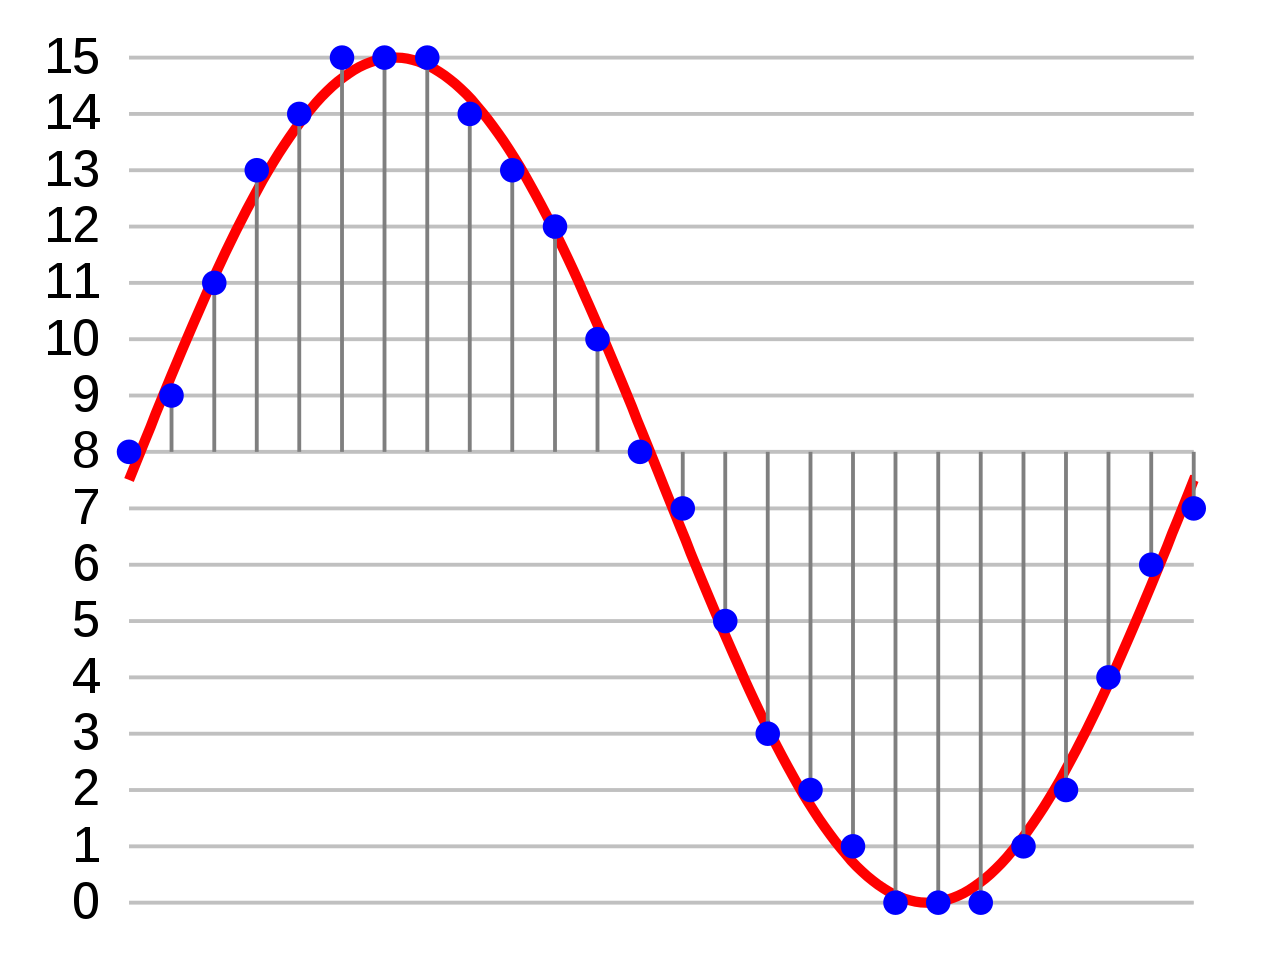
\includegraphics[width=12cm]{images/son}
\end{figure}
\end{center}

Ce processus est nommé l'échantillonnage et on échantillonne en général les sons à 44 kHz (ce qui correspond à une valeur toutes les 1/44000 secondes, soit toutes les 23 $\mu s$), soit 2x plus que le son le plus aigu que l'oreille humaine peut entendre (22kHz).

\subsubsection{Les formats audios}
\begin{enumerate}
\item Cette technique est celle utilisée dans certains formats de sons "bruts" comme le RAW ou WAV. 

\item D'autres formats, comme le MP3, compressent encore ces informations, comme le fait le JPG pour les images.

\item D'autres formats, comme le MIDI, n'utilisent pas cette méthode et font le choix de noter directement l'équivalent des notes de musique et des instruments sur lesquels elles sont jouées. Ce format est adapté aux musiques composées sur synthétiseurs, mais pas aux sons enregistrés dans la nature.

\end{enumerate}

\section{Exercices}


\iffalse   %%%%%%% Commented --> move to ch1
\begin{exercice}
Traduire les mots suivants en code ASCII binaire :
\begin{enumerate}
\item \#MeToo
\item 2+2<5
\end{enumerate}
\end{exercice}

\begin{exercice}
Traduire en lettres la phrase suivante qui est codée en ASCII (binaire):
\begin{enumerate}
\item 01000011 01100001 00100000 01100011 00100111 01100101 01110011 01110100 00100000 01100100 01110101 00100000 01100010 01101001 01101110 01100001 01101001 01110010 01100101 00101110
\end{enumerate}
\end{exercice}

\begin{exercice}
Traduire en lettre les mots suivants qui sont codés en ASCII (hexadécimal):
\begin{enumerate}
\item 42696E76656E7521
\item 31323D332A342C204F4B3F
\end{enumerate}
\end{exercice}
\fi 

\begin{exercice}
Décoder l'image suivante:

\begin{center}
\begin{tikzpicture}[scale=.5]
\foreach \x in {0,...,16}{
	\draw (\x,0) -- +(0,13);
	}

\foreach \x in {0,...,13}{
	\draw (0,\x) -- +(16,0);
	}

\draw (17,12.5) node[right] {6,5,2,3}; 
\draw (17,11.5) node[right] {4,2,5,2,3,1}; 
\draw (17,10.5) node[right] {3,1,9,1,2,1}; 
\draw (17,9.5) node[right] {3,1,9,1,1,1}; 
\draw (17,8.5) node[right] {2,1,11,1}; 
\draw (17,7.5) node[right] {2,1,10,2}; 
\draw (17,6.5) node[right] {2,1,9,1,1,1}; 
\draw (17,5.5) node[right] {2,1,8,1,2,1}; 
\draw (17,4.5) node[right] {2,1,7,1,3,1}; 
\draw (17,3.5) node[right] {1,1,1,1,4,2,3,1}; 	
\draw (17,2.5) node[right] {0,1,2,1,2,2,5,1}; 	
\draw (17,1.5) node[right] {0,1,3,2,5,2}; 	
\draw (17,0.5) node[right] {1,3,2,5}; 	

\end{tikzpicture}
\end{center}
\end{exercice}

%\newpage
\begin{exercice}
Encoder l'image suivante:

\begin{center}
\begin{figure}[h!]
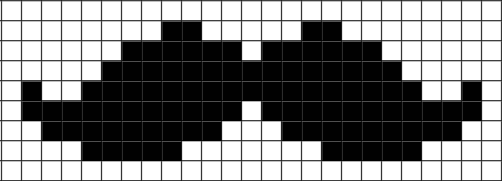
\includegraphics[width=8cm]{images/moustache}
\end{figure}
\end{center}

\end{exercice}



\begin{exercice}
    
Combien d’octets occupe une image de 200 x 300 pixels en noir et blanc?
\end{exercice}

\begin{exercice}
\begin{enumerate}
\item 
    Combien d'octets occupe une image de 300 x 500 pixels en niveau de gris codé sur 8 bits ?
      \item
        Même question, mais si on a une en couleur pour laquelle chaque couleur est codée en RVB sur 24 bits
\end{enumerate}

\end{exercice}


\begin{exercice}
\begin{enumerate}
    \item Combien de niveaux de gris pourrait-on encoder sur 10 bits ?
    
    \item Sur 8 bits, quel gris est le plus foncé entre celui représenté par la valeur 42 et celui représenté par la valeur 233 ? 

    \item Quel est d'après vous le code RGB du violet foncé ? %160-0-160

    \item Quelle est d'après vous la couleur correspondant au code RGB suivant : (255, 128, 0) ? % orange
\end{enumerate}
\end{exercice}

\begin{exercice}
Si une image codée en RVB (RGB) de 16,7 millions de couleurs occupe 2400 octets, de combien de pixels sera-t-elle constituée ?
\end{exercice}


\begin{exercice}
 * J’aimerais imprimer une image full hd (1920 x 1080 pixels) sur mon imprimante qui a une résolution de 1200 dpi. 
Quelles seront les dimensions en centimètre (largeur et hauteur) ?

\end{exercice}



\end{document}